\documentclass[spanish]{beamer}

%%% CODIFICACIÓN

\usepackage[utf8]{inputenc}
\usepackage[spanish]{babel}
\usepackage{graphics,tikz}
\graphicspath{{./fig/}}
\usepackage{caption}
\usepackage{subcaption}
%%% FUENTES

\usepackage[T1]{fontenc}
\usepackage[familydefault,regular]{}
\usepackage{newtxsf} % Fuente de matemáticas

\setbeamertemplate{navigation symbols}{}

%%% COLORES

\definecolor{background}{RGB}{255,255,255}
\definecolor{text}{RGB}{78,78,78}
\definecolor{accent}{RGB}{6, 105, 125}

\setbeamerfont{framesubtitle}{size=\normalfont\tiny}
\setbeamercolor{framesubtitle}{fg=white}

%%% Matemáticas
\usepackage{amsmath}
\usepackage{amssymb}
\usepackage{amsbsy}
\usepackage{tipa}
\newcommand{\norm}[1]{\left\lVert#1\right\rVert}
\newcommand{\yy}{\textbf{y}}
\usepackage{blkarray}

%%% Código
\usepackage{listings}

%%% Tablas
\usepackage{tabularx}
\usepackage{float}
\usepackage{adjustbox}
\usepackage{booktabs}
\usepackage{array}
\newcolumntype{L}[1]{>{\raggedright\let\newline\\\arraybackslash\hspace{0pt}}m{#1}}
\newcolumntype{C}[1]{>{\centering\let\newline\\\arraybackslash\hspace{0pt}}m{#1}}
\newcolumntype{R}[1]{>{\raggedleft\let\newline\\\arraybackslash\hspace{0pt}}m{#1}}
\usepackage{multirow}

%%% AJUSTES DE BEAMER

% ¿Negrita en el título de diapositiva o no?
%\setbeamertemplate{frametitle}{\color{accent}\vspace*{1cm}\bfseries\insertframetitle\par\vskip-6pt}

\setbeamertemplate{frametitle}{\color{accent}\vspace*{1cm}\insertframetitle\par\vskip-6pt}

\setbeamertemplate{itemize items}[circle] % Viñetas de itemize

%%% CONFIGURACIÓN DE COLORES DE BEAMER

\setbeamercolor{background canvas}{bg=background}
\setbeamercolor{normal text}{fg=text}
\setbeamercolor{alerted text}{fg=accent}
\setbeamercolor{block title}{fg=accent}
\setbeamercolor{alerted text}{fg=accent}
\setbeamercolor{itemize item}{fg=accent}
\setbeamercolor{enumerate item}{fg=accent}
\setbeamercolor*{title}{fg=accent}
\setbeamercolor{caption name}{fg=accent}
\setbeamercolor{qed symbol}{fg=accent}
\setbeamercolor{itemize subitem}{fg=accent}
\setbeamercolor{bibliography entry author}{fg=text}
\setbeamertemplate{itemize subitem}[triangle]
\usebeamercolor[fg]{normal text}

%%% SECTIONS
\setbeamercolor{mycolor}{fg=white,bg=accent}

\AtBeginSection[]{
  \begin{frame}
  \vfill
  \centering
  \begin{beamercolorbox}[sep=8pt,center,shadow=true,rounded=true]{mycolor}%
    \usebeamerfont{title}\insertsectionhead\par%
  \end{beamercolorbox}
  \vfill
  \end{frame}
}



%%% INFORMACIÓN DEL DOCUMENTO

\title{\textit{Clustering}}
\subtitle{Estadística Multivariante}
\author{Sofía Almeida Bruno\\ Daniel Bolaños Martínez\\ José María Borrás Serrano\\ Fernando de la Hoz Moreno\\ Pedro Manuel Flores Crespo\\ María Victoria Granados Pozo}


\begin{document}

\maketitle
	
\begin{frame}{\textit{Clustering}}
  \begin{itemize}
  \item Objetivo: agrupar objetos similares.\break
  \item Dadas \textbf{$x_1$}$,\cdots, $\textbf{$x_n$} medidas de $p$ variables en $n$ objetos considerados \textit{heterogéneos}. El objetivo del análisis clúster es agrupar estos objetos en $k$ clases \textit{homogéneas}, donde $k$ es también desconocido.
  \end{itemize}
\end{frame}

\begin{frame}{\textit{Clustering}}
\begin{figure}[H]
	\centering
	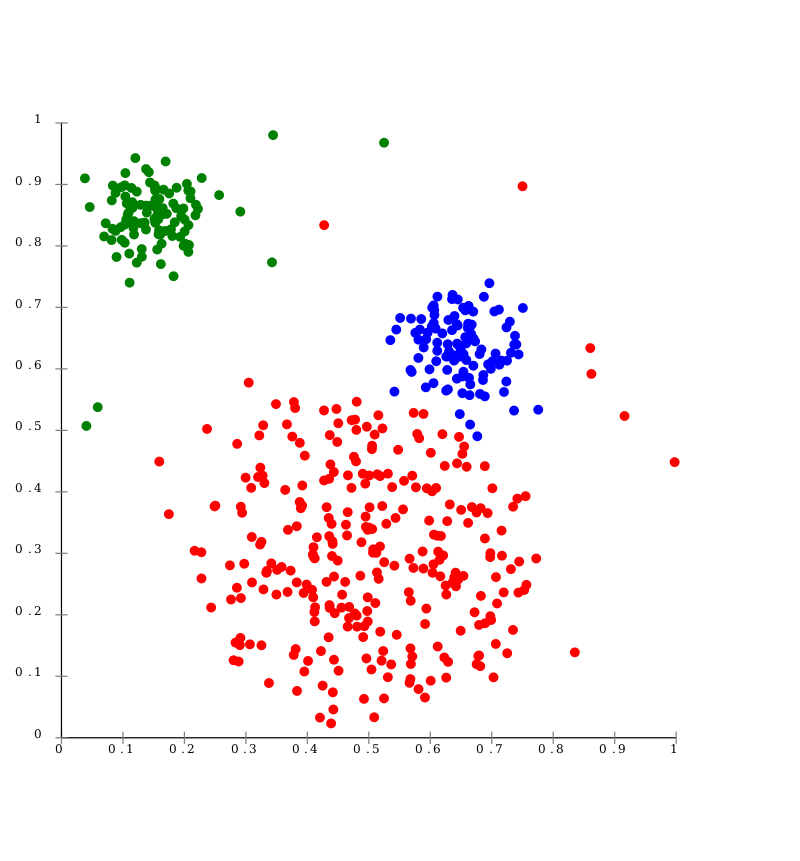
\includegraphics[scale=0.2]{ejemplo}
	\caption{Ejemplo de \textit{clustering}. \cite{chire_deutsch:_2011}}
	\label{fig:ejemplo1}
\end{figure}
\end{frame}

\begin{frame}{Ejemplos de \textit{Clustering}}
  \begin{itemize}
  \item Biología: determinación de especies.
  \item \textit{Marketing}: descubrimiento de grupos de clientes.
    \begin{figure}[H]
	\centering
	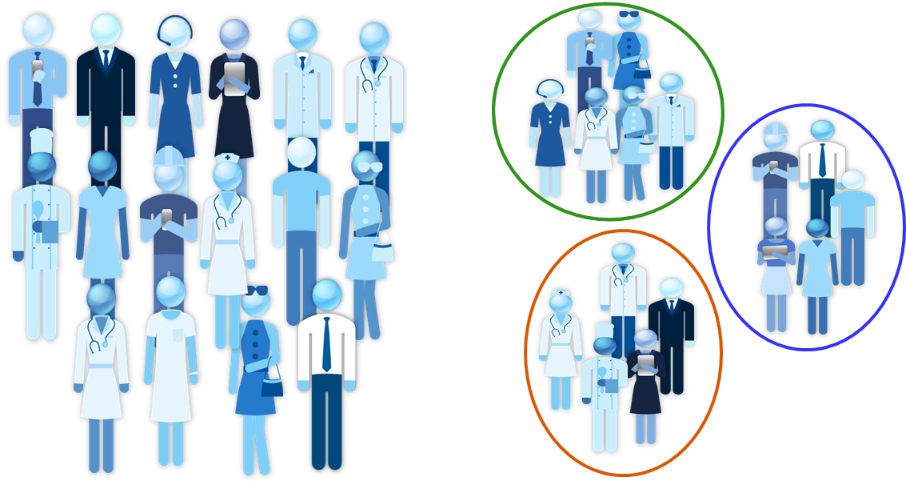
\includegraphics[scale=0.5]{ej_marketing}
	\caption{Ejemplo de \textit{clustering}. \cite{noauthor_understanding_nodate}}
\end{figure}
  \item Psicología: encontrar tipos de personalidad.
  \item Arqueología: datar objetos encontrados.
  \item Planificación urbana: identificar grupos de viviendas.
  \end{itemize}
\end{frame}

\begin{frame}{\textit{Clustering}}
  Para realizar un análisis clúster hay que:\break
  \begin{itemize}
  \item Elegir una medida de similitud.\break
  \item Elegir un algoritmo para construir los grupos.
    \begin{itemize}
    \item Particionamiento.
    \item Jerárquicos.
    \end{itemize}
  \end{itemize}
\end{frame}

\section{Medidas de similitud}

\begin{frame}{Medidas de similitud}

Consideraciones iniciales como:\break

\begin{itemize}
\item Naturaleza de las variables (discreta, continua, binaria).
\item Escalas de las medidas (nominal, ordinal, intervalo).
\item Conocimiento sobre el problema.
\end{itemize}\

Los valores de las variables consideradas deberán ser normalizados.
\end{frame}

\begin{frame}{Distancias de similitud para pares de ítems}

La distancia estadística entre dos observaciones $p$-dimensionales $x^T = [x_1,\dots,x_p]$ e $y^T=[y_1,\dots,y_p]$ es:

$$d(x,y)=\sqrt{(x-y)^TA(x-y)}. $$

Donde: \break
\begin{itemize}
\item $A=S^{-1}$. 
\item $S$ contiene las varianzas y covarianzas de la muestra.
\end{itemize}
\end{frame}

\begin{frame}{Otras medidas y coeficientes de similitud}

\begin{itemize}
\item Métrica de Minkowski:
$$ d(x,y)=\left  [\sum_{i=1}^{p}{|x_i-y_i|^m} \right ]^{1/m}.$$
\item Métrica de Canberra (variables no negativas):
$$d(x,y)=\sum_{i=1}^{p}{\frac{|x_i-y_i|}{(x_i+y_i)}}.$$
\item Coeficiente de Czekanowski (variables no negativas):
$$d(x,y)=1-\frac{2\sum_{i=1}^{p}{min(x_i,y_i)}}{\sum_{i=1}^{p}{(x_i+y_i}}.$$
\end{itemize}
\end{frame}

%% \begin{frame}{Propiedades distancia ''verdadera''}
%% \begin{itemize}
%% \item $d(P,Q)=d(Q,P)$.
%% \item $d(P,Q)>0\ si\ P\neq Q$.
%% \item $d(P,Q)=0\ si\ P=Q$.
%% \item $d(P,Q)\leq d(P,R)+d(R,Q)$.
%% \end{itemize}\

%% con $P$ y $Q$ dos puntos y $R$ su punto intermedio.\break

%% La mayoría de algoritmos de clustering aceptan distancias que no satisfagan la desigualdad triangular.
%% \end{frame}

%% \begin{frame}{Binarización de variables}

%% Si los ítems no pueden ser representados por medidas $p$-dimensionales significativas, las parejas de ítems se suelen comparar según la \textbf{presencia o ausencia} de ciertas características.\break

%% Matemáticamente se consigue introduciendo una variable binaria, que toma el valor \textbf{1} si la característica \textbf{está presente} y el valor \textbf{0} si \textbf{no}. 
%% \end{frame}

\begin{frame}{Frecuencias de las parejas}

Organizamos las frecuencias en la siguiente \textbf{tabla de contingencia}:\break

\begin{table}[h]
  \centering
  \label{tab:contingencia_var}
\resizebox{8cm}{!} {
\begin{tabular}{llrrrr}
\toprule
\multicolumn{2}{l}{\multirow{2}{*}{}} & \multicolumn{2}{c}{Ítem $k$} & \multicolumn{2}{c}{\multirow{2}{*}{Total}} \\\cmidrule{3-4}
\multicolumn{2}{l}{}                  & 1             & 0       & \multicolumn{2}{c}{}                        \\ \hline
\multirow{2}{*}{Ítem $i$}       & 1     & $a$          & $b$       & \multicolumn{2}{c}{$a+b$}                     \\
                              & 0      & c            & $d$       & \multicolumn{2}{c}{$c+d$}                     \\ \hline
\multicolumn{2}{l}{Total}            & $a+c$          & $b+d$     & \multicolumn{2}{c}{$p=a+b+c+d$}\\
\bottomrule            
\end{tabular}
}
\end{table}

\end{frame}

\begin{frame}{Coeficientes de similitud para ítems \textit{clustering}}

\begin{table}[H]
  \centering
\resizebox{11cm}{!} {
\begin{tabular}{ll}
\toprule               
\multicolumn{1}{l}{Coeficiente} & \multicolumn{1}{l}{Fundamento}\\
\midrule
1 $\quad\frac{a+d}{p}$                            & Las parejas 1-1 y 0-0 ponderan lo mismo.\\ \\
2 $\quad\frac{2(a+d)}{2(a+d)+b+c}$                            & Las parejas 1-1 y 0-0 ponderan el doble.                                                                                                        \\\\
3 $\quad\frac{a+d}{a+d+2(b+c)}$                             & Las parejas que no coinciden ponderan el doble.                                                                                                 \\\\
4  $\quad\frac{a}{p}$                             & No hay parejas 0-0 en el numerador.                                                                                                    \\         \\
\bottomrule
\end{tabular}
}
\end{table}

\end{frame}

\begin{frame}{Coeficientes de similitud para ítems \textit{clustering}}
\begin{table}[H]
  \centering
\resizebox{11cm}{!} {
\begin{tabular}{ll}
\toprule               
\multicolumn{1}{l}{Coeficiente} & \multicolumn{1}{l}{Fundamento}\\
\midrule
5 $\quad\frac{a}{a+b+c}$                             & \begin{tabular}[c]{@{}l@{}}No hay parejas 0-0 en el numerador ni el denominador\\ (Las parejas 0-0 son irrelevantes).\end{tabular}              \\\\
6 $\quad\frac{2a}{2a+b+c}$                             & \begin{tabular}[c]{@{}l@{}}No hay parejas 0-0 en el numerador ni el denominador.\\ Las parejas 1-1 ponderan el doble.\end{tabular}              \\\\
7 $\quad\frac{a}{a+2(b+c)}$                             & \begin{tabular}[c]{@{}l@{}}No hay parejas 0-0 en el numerador ni el denominador.\\ Las parejas que no coinciden ponderan el doble.\end{tabular} \\\\
8 $\quad\frac{a}{b+c}$                             & \begin{tabular}[c]{@{}l@{}}Proporción de parejas que coinciden (excluyendo las 0-0) en\\  relación a las parejas que no coinciden.\end{tabular} \\\\
\bottomrule
\end{tabular}
}
\end{table}
\end{frame}

\begin{frame}{Construcción de similitudes y distancias}
\begin{itemize}
\item Siempre se pueden construir similitudes a partir de distancias.\break

Fijando $ s_{ik} = \frac{1}{1+d_{ik}}$ donde $0<s_{ik}\leq 1$ es la similitud entre los ítems $i$ y $k$, entonces $d_{ik}$ es la distancia correspondiente.\break

\item Las distancias se pueden construir a partir de similitudes si la matriz de similitudes es definida no negativa y la máxima similitud cumple $s_{ii}=1$.\break

Entonces $ d_{ik}=\sqrt{2\cdot(1-s_{ik})}$, cumple las propiedades de una distancia.
\end{itemize}
\end{frame}

\begin{frame}{Medidas de similitud para pares de variables}
Las medidas de similitud para variables suelen tomar la forma de coeficientes de correlaciones muestrales.\break

Cuando las variables son binarias, los datos se pueden organizar en una \textbf{tabla de contingencia} que tiene la siguiente forma:
\begin{table}[h]
  \centering
  \label{tab:contingencia_var}
\resizebox{7.5cm}{!} {
\begin{tabular}{llrrrr}
\toprule
\multicolumn{2}{l}{\multirow{2}{*}{}} & \multicolumn{2}{c}{Variable $k$} & \multicolumn{2}{c}{\multirow{2}{*}{Total}} \\\cmidrule{3-4}
\multicolumn{2}{l}{}                  & 1             & 0       & \multicolumn{2}{c}{}                        \\ \hline
\multirow{2}{*}{Variable $i$}       & 1      & $a$          & $b$       & \multicolumn{2}{c}{$a+b$}                     \\
                              & 0      & c            & $d$       & \multicolumn{2}{c}{$c+d$}                     \\ \hline
\multicolumn{2}{l}{Total}            & $a+c$          & $b+d$     & \multicolumn{2}{c}{$n=a+b+c+d$}\\
\bottomrule            
\end{tabular}
}
\end{table}
\end{frame}

\begin{frame}{Medidas de similitud para pares de variables}
La fórmula del coeficiente de correlación producto-momento aplicada a las variables binarias de la tabla de contingencia nos da:\break

$$r = \frac{ad-bc}{[(a+b)(c+d)(a+c)(b+d)]^{1/2}}.$$\

$r$ se puede tomar como la medida de similitud entre las dos variables.
\end{frame}

\begin{frame}{Ejemplo idiomas}
Medimos las similitudes de 11 lenguajes en base a los primeros 10 números naturales en cada idioma.

\begin{table}[h]
\centering
\resizebox{11.3cm}{!} {
  \begin{tabular}{lllllllllll}
    \toprule
\begin{tabular}[c]{@{}l@{}}Inglés\\ (E)\end{tabular} & \begin{tabular}[c]{@{}l@{}}Noruego\\ (N)\end{tabular} & \begin{tabular}[c]{@{}l@{}}Danés\\ (Da)\end{tabular} & \begin{tabular}[c]{@{}l@{}}Holandés\\ (Du)\end{tabular} & \begin{tabular}[c]{@{}l@{}}Alemán\\ (G)\end{tabular} & \begin{tabular}[c]{@{}l@{}}Francés\\ (Fr)\end{tabular} & \begin{tabular}[c]{@{}l@{}}Español\\ (Sp)\end{tabular} & \begin{tabular}[c]{@{}l@{}}Italiano\\ (I)\end{tabular} & \begin{tabular}[c]{@{}l@{}}Polaco\\ (P)\end{tabular} & \begin{tabular}[c]{@{}l@{}}Húngaro\\ (H)\end{tabular} & \begin{tabular}[c]{@{}l@{}}Finés\\ (Fi)\end{tabular} \\ \midrule
one                                                  & en                                                    & en                                                   & een                                                     & eins                                                 & un                                                     & uno                                                    & uno                                                    & jeden                                                & egy                                                   & yksi                                                 \\
two                                                  & to                                                    & to                                                   & twee                                                    & zwei                                                 & deux                                                   & dos                                                    & due                                                    & dwa                                                  & ketto                                                 & kaksi                                                \\
three                                                & tre                                                   & tre                                                  & drie                                                    & drei                                                 & trois                                                  & tres                                                   & tre                                                    & trzy                                                 & harom                                                 & kolme                                                \\
four                                                 & fire                                                  & fire                                                 & vier                                                    & vier                                                 & quatre                                                 & cuatro                                                 & quattro                                                & cztery                                               & negy                                                  & nelja                                                \\
five                                                 & fem                                                   & fem                                                  & vijf                                                    & funf                                                 & cinq                                                   & cinco                                                  & cinque                                                 & piec                                                 & ot                                                    & viisi                                                \\
six                                                  & seks                                                  & seks                                                 & zes                                                     & sechs                                                & six                                                    & seis                                                   & sei                                                    & szesc                                                & hat                                                   & kuusi                                                \\
seven                                                & sju                                                   & syv                                                  & zeven                                                   & sieben                                               & sept                                                   & siete                                                  & sette                                                  & siedem                                               & het                                                   & seitseman                                            \\
eight                                                & atte                                                  & otte                                                 & acht                                                    & acht                                                 & huit                                                   & ocho                                                   & otto                                                   & osiem                                                & nyolc                                                 & kahdeksan                                            \\
nine                                                 & ni                                                    & ni                                                   & negen                                                   & neun                                                 & neuf                                                   & nueve                                                  & nove                                                   & dziewiec                                             & kilenc                                                & yhdeksan                                             \\
ten                                                  & ti                                                    & ti                                                   & tien                                                    & zehn                                                 & dix                                                    & diez                                                   & dieci                                                  & dziesiec                                             & tiz                                                   & kymmenen                                             \\ \bottomrule
\end{tabular}
}
\end{table}
\end{frame}

\begin{frame}{}
\begin{table}[h]
\centering
\makebox[\textwidth][c]{
\begin{tabular}{lrrrrrrrrrrr}
\\
\toprule
       & E      & N      & Da     & Du     & G     & Fr    & Sp    & I     & P     & H     & Fi    \\ \midrule
E      & 10     &        &        &        &       &       &       &       &       &       &       \\
N      & 8      & 10     &        &        &       &       &       &       &       &       &       \\
Da     & 8      & 9      & 10     &        &       &       &       &       &       &       &       \\
Du     & 3      & 5      & 4      & 10     &       &       &       &       &       &       &       \\
G      & 4      & 6      & 5      & 5      & 10    &       &       &       &       &       &       \\
Fr     & 4      & 4      & 4      & 1      & 3     & 10    &       &       &       &       &       \\
Sp     & 4      & 4      & 5      & 1      & 3     & 8     & 10    &       &       &       &       \\
I      & 4      & 4      & 5      & 1      & 3     & 9     & 9     & 10    &       &       &       \\
P      & 3      & 3      & 4      & 0      & 2     & 5     & 7     & 6     & 10    &       &       \\
H      & 1      & 2      & 2      & 2      & 1     & 0     & 0     & 0     & 0     & 10    &       \\
Fi     & 1      & 1      & 1      & 1      & 1     & 1     & 1     & 1     & 1     & 2     & 10    \\ \bottomrule
\end{tabular}
}
\end{table}\

Vemos que inglés, noruego, danés, holandés y alemán parecen formar un grupo. El francés, español, italiano y polaco forman otro, mientras que el húngaro y el finés no forman parte de ninguno.
\end{frame}

\section{Métodos de agrupamiento}
\begin{frame}{Métodos de agrupamiento}
  \textbf{Definición:} procedimiento de agrupación de una serie de vectores de acuerdo con un criterio (distancia o similitud).\break
  
\textbf{Tipos:}
	\begin{itemize}
		\item Jerárquicos.
		\item No jerárquicos o particionamiento.
	\end{itemize}
\end{frame}

\begin{frame}{Métodos de agrupamiento}
	
	\begin{figure}[H]
		\centering
		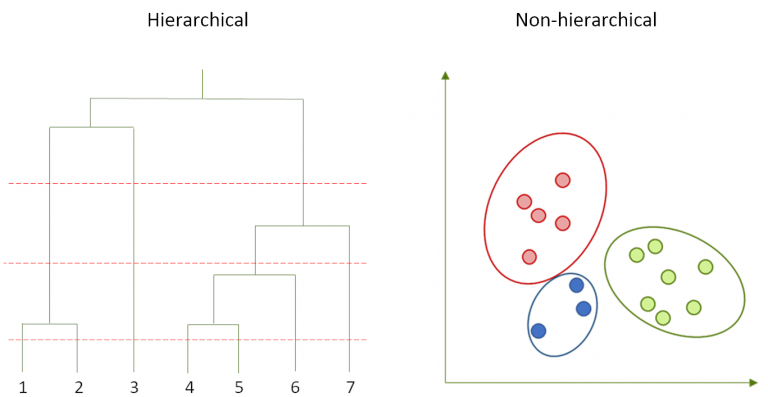
\includegraphics[scale=0.5]{victoria/compJerarquicoNoJerarquico}
		\caption{Comparación métodos jerárquico y no jerárquico.}
		\label{fig:ejemplo_metodos}
	\end{figure}

\end{frame}

\section{Métodos de agrupamiento\\ Jerárquicos}
\begin{frame}{Métodos Jerárquicos}
	\begin{figure}[H]
		\centering
		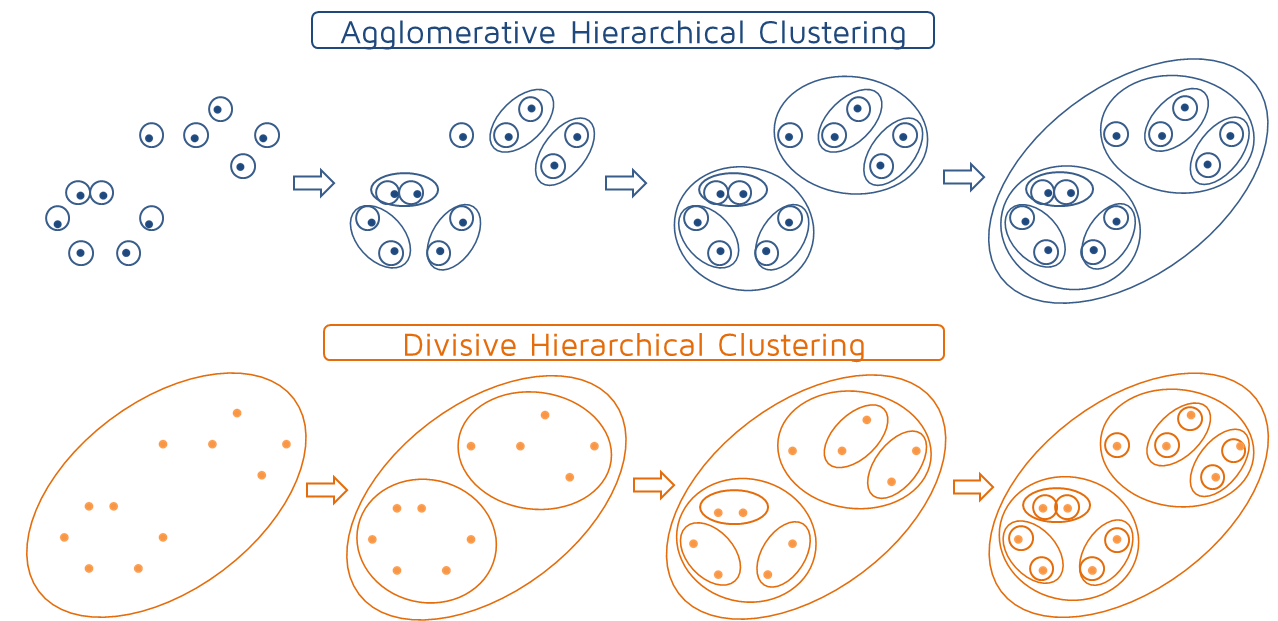
\includegraphics[scale=0.23]{victoria/compAglomeDivisivo}
		\caption{Comparación métodos aglomerativos y divisivos.}
		\label{fig:agl_div}
	\end{figure}
\end{frame}

\begin{frame}{Comparación de técnicas aglomerativas y divisivas}

	\begin{figure}[H]
	\centering
	\begin{subfigure}[b]{.47\textwidth}
		  \centering
	  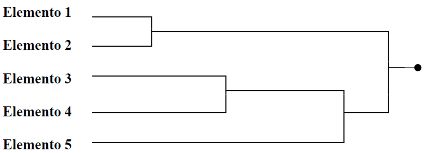
\includegraphics[width=\textwidth]{victoria/aglomerativo}
	  \caption{Dendrograma aglomerativo.}
	  \label{fig:aglomerativo}
	\end{subfigure}
	\begin{subfigure}[b]{.47\textwidth}
	  \centering
	  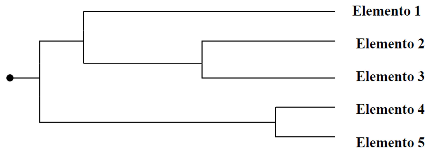
\includegraphics[width=\textwidth]{victoria/disociativo}
	  \caption{Dendrograma divisivo.}
	  \label{fig:divisivo}
	\end{subfigure}
	\label{fig:compDendro}
	\end{figure}

\end{frame}

\begin{frame}{Ejemplo \textit{Single Link Method}}

	\textbf{Distancia entre dos clústers}

	\begin{equation}\label{eq:distAgloEjm}
		d(R, S) = min \{d_{rs}\ :\ r \in R, \ s \in S\}.
	\end{equation}
\textbf{Matriz de distancias}
	\[ \mathcal{D} =
	\left[ \begin{array}{c}
	d_{rs}
	\end{array} \right] =
	\begin{blockarray}{cccccc}
		& 1 & 2 & 3 & 4 & 5 \\
		\begin{block}{c[ccccc]}
			\\
			1 & 0 & \textbf{2} & 4 & 7 & 9 \\
			2 & \textbf{2} & 0 & 8 & 9 & 8 \\
			3 & 4 & 8 & 0 & 3 & 7 \\
			4 & 7 & 9 & 3 & 0 & 5 \\
			5 & 9 & 8 & 7 & 5 & 0 \\
			\\
		\end{block}
	\end{blockarray}  .
	\] 

\end{frame}


\begin{frame}{Ejemplo \textit{Single Link Method}}

	Cálculo de las nuevas distancias:
	\begin{center}
	$d_{(12)(3)}$ = min\{$d_{13}$, $d_{23}$\} = min \{4, 8\} = 4,\\
	$d_{(12)(4)}$ = min\{$d_{14}$, $d_{24}$\} = min \{7, 9\} = 7,\\
	$d_{(12)(5)}$ = min\{$d_{15}$, $d_{25}$\} = min \{9, 8\} = 8.\\
	\end{center}
	\textbf{Matriz de distancias}
	\[ \mathcal{D}_1  =
	\begin{blockarray}{ccccc}
		& (12) & 3 & 4 & 5 \\
		\begin{block}{c[cccc]}
			\\
			(12) & 0 & 4 & 7 & 8 \\
			3 & 4 & 0 & \textbf{3} & 7 \\
			4 & 7 & \textbf{3} & 0 & 5 \\
			5 & 8 & 7 & 5 & 0 \\
			\\
		\end{block}
	\end{blockarray} . 
	\]
\end{frame}

\begin{frame}{Ejemplo \textit{Single Link Method}}

	Cálculo de las nuevas distancias:\\
	\begin{center}
		$d_{(34)(12)}$ = min\{$d_{(3)(12)}$, $d_{(4)(12)}$\} = min \{4, 7\} = 4,\\
		$d_{(34)(5)}$ = min\{$d_{(3)(5)}$, $d_{(4)(5)}$\} = min \{7, 5\} = 5.\\
	\end{center}
	\textbf{Matriz de distancias}
	\[ \mathcal{D}_2  =
	\begin{blockarray}{cccc}
		& (12) & (34) & 5 \\
		\begin{block}{c[ccc]}
			\\
			(12) & 0 & \textbf{4} & 8 \\
			(34) & \textbf{4} & 0 & 5 \\
			5 & 8 & 5 & 0 \\
			\\
		\end{block}
	\end{blockarray}  .
	\] 
\end{frame}

\begin{frame}{Ejemplo \textit{Single Link Method}}

	Cálculo de la nueva distancia:
	\begin{center}
	$d_{(12)(34)5}$ = min\{$d_{(12)(5)}$, $d_{(34)(5)}$\} = min \{8, 5\} = 5.
	\end{center}
	Finalmente se obtiene el clúster \textit{(12345)}.
%% \end{frame}

%% \begin{frame}{Ejemplo \textit{Single Link Method}}
	\begin{figure}[H]
		\centering
		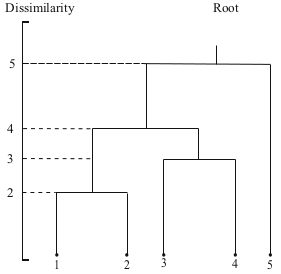
\includegraphics[scale=0.48]{victoria/agloEjem}
		\label{fig:agloEjem}
	\end{figure}
\end{frame}

\section{Métodos de agrupamiento\\ Particionamiento}

%% \begin{frame}{Particionamiento}
%%   \begin{itemize}
%%   \item No hay dependencia jerárquica entre soluciones.
%%   \item Se explora un número limitado de agrupaciones.
%%   \item Se busca maximizar la similitud en los clústeres.
%%   \end{itemize}

%% \end{frame}



\begin{frame}{\textit{K-medias}}
\begin{enumerate}
\item Entrada: $\textbf{L}=\{\textbf{x}_i,i=1,2,...,n\}$, K=número de clústeres.

\item Hacer uno de los siguientes:
\begin{itemize}
\item Formar una asignación aleatoria inicial de los datos en los K clústeres y, para los K clústeres, calcular su centroide, $\overline{\textbf{x}}_k, k=1,2,...,K$.
\item Pre-especificar los centroides de los K clústeres, $\overline{\textbf{x}}_k, k=1,2,...,K$.
\end{itemize}
\item Calcular la distancia euclídea al cuadrado para cada dato al centroide de su clúster actual:
$$ESS=\sum_{k=1}^{K}\sum_{c(i)=k}(\textbf{x}_i - \overline{\textbf{x}}_k)^T(\textbf{x}_i - \overline{\textbf{x}}_k)$$

donde $\overline{\textbf{x}}_k$ es el centroide del $k$-ésimo clúster y $c(i)$ es el clúster que contiene $\textbf{x}_i$.

\end{enumerate}
\end{frame}


\begin{frame}{\textit{K-medias}}
\begin{enumerate}

\item[$4.$] Reasignamos cada dato al clúster con el centroide más cercano de tal manera que ESS se reduce en magnitud. Actualizamos los centroides de los clústeres después de la reasignación de los datos. 
\item[$5.$] Repetimos los pasos 3 y 4 hasta que no se produzcan más reasignaciones.
\end{enumerate}

\end{frame}

\begin{frame}{Otros métodos de particionamiento}
K-Medoides:
\begin{itemize}
\item Medoide: dato más representativo del clúster.
\item No se utiliza la distacia euclídea.
\end{itemize}
PAM:
\begin{itemize}
\item Modificación de K-Medoides.
\end{itemize}
Análisis difuso:
\begin{itemize}
\item Se asigna una probabilidad de pertenecer a cada clúster.
\end{itemize}
Mean Shift:
\begin{itemize}
\item Método iterativo que parte de una estimación inicial $x$.
\item Localiza los máximos de una función de densidad.
 \end{itemize}
\end{frame}

\begin{frame}{DBSCAN}
\begin{itemize}
\item Se basa en la densidad de las muestras para identificar los clústeres.
  \begin{figure}[h]
\centering
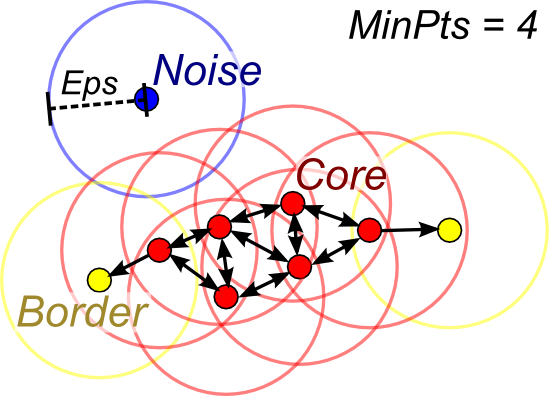
\includegraphics[scale=1.]{dani/DBSCAN.png}
\end{figure}

\item Todos los puntos de un mismo clúster están conectados entre sí.
\item Si un punto $A$ es alcanzable desde cualquier otro punto $B$ del clúster, entonces $A$ también forma parte del clúster.
\end{itemize}

\end{frame}


\section{Número de clústeres}

\begin{frame}{Método del codo}
	Consiste en dibujar la gráfica de las distancia a los centros de cada clúster en función del número de clústeres. Definimos:
	\[
	SSE_k = \sum_{i = 1}^{n_k} \norm{\yy_i - \bar{\yy}_k}^2,
	\]
	y para cada $ k $ dibujamos
	\[
	D_k = \sum_{i = 1} ^ {k} SSE_k.
	\]
\end{frame}

\begin{frame}{Método del codo}
	\begin{figure}[h]
		\centering
		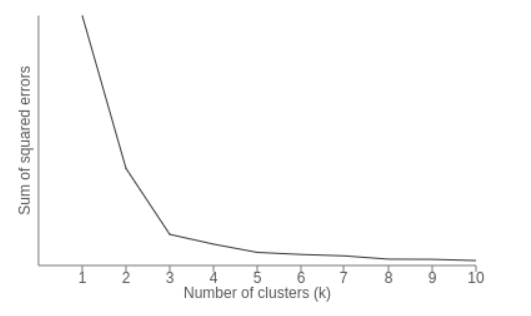
\includegraphics[scale=0.5]{pedro/elbowGraph}
		\caption{Ejemplo del método del codo \cite{elbowGraph}.}
		\label{smkm}
	\end{figure}
\end{frame}

\begin{frame}{Estadístico $ R^2 $}
	Para $ n $ clústeres la suma total de las distancias al cuadrado es $ T = \sum_{i = 1}^{n} \norm{\yy_i - \bar{\yy}}^2 $. Así, para $ k $ clústeres definimos $ R^2 $ como
	\[
	R^{2}_{k} = \frac{T - \sum_k SSE_k}{T}.
	\]
	Para $ n $ clústeres $ SSE_k = 0 $ por lo que $ R^2 = 1 $. Una gran disminución en $ R^2_k $ representaría un mal agrupamiento. \break
       
También podríamos tener en cuenta el cambio en $ R^2 $ al unir los clústeres $ R $ y $ S $ como $ SR^2 = R_k^2 - R^2_{k-1} $.
\end{frame}

\begin{frame}{Varianza agrupada}
	Para un solo clúster \[ s^2 = \sum_{i=1}^{n} \norm{\yy_i - \bar{\yy}}^2/ p(n-1).\]
	Para el clúster $ C_k $
	\[
	s^2 = \sum_{i=1}^{n_k} \norm{\yy_i - \bar{\yy}_k}^2/ p(n_k-1).
	\]
	Valores grandes de la varianza agrupada indica que los clústeres no son homogéneos. Por lo tanto, si tiende a cero para algún $  k < n $ indica la formación de un clúster homogéneo.
\end{frame}

\begin{frame}{Pseudo estadísticos}
	El pseudo estadístico $ F $ se define como
	\[
	F^*_k = \frac{(T-\sum_k SSE_k) / (k-1)}{\sum_k SSE_k / (n-k)}.
	\]
	El pseudo estadístico $ t^2 $ se define como
	\[
	\text{pseudo }t^2 = \frac{\lbrack SSE_t - (SSE_r + SSE_s)\rbrack(n_R + n_S - 2)}{SSE_r + SSE_s}.
	\]
\end{frame}

\begin{frame}{\textit{Silhouette method}}
	Definimos el índice:
	\[
	s(i) = \frac{b(i)-a(i)}{\max\{b(i), a(i)\}}, \hspace{2mm} \forall i = 1, \dots, n
	\] 
	donde 
	\[
	a(i) = \frac{1}{|C_i|-1}\sum_{j\in C_i, j \neq i} d(i,j) 
	\]	y
	\[
	b(i) = \min_{k \neq i} \frac{1}{|C_k|} \sum_{j \in C_k} d(i,j).
	\] 
	Se escoge el $ k $ que maximice el valor medio de $ s(i) $.
\end{frame}

\begin{frame}{\textit{Silhouette method}}
	\begin{table}[h!]
		\centering
		\begin{tabular}{cc} 
			\hline
			k & Silhouette coeff. \\
			\hline
			2 &  0.7049787496083262 \\			 
			3 & 0.5882004012129721 \\	
			4 &  0.6505186632729437 \\
			5 &  0.5745566973301872 \\
			6 & 0.43902711183132426 \\
			\hline
		\end{tabular}
		\caption{Ejemplo \textit{silhouette method} \cite{silouetteGraph}.}
	\end{table}
	Vemos que se obtienen los mejores resultados con 2 o 4 clústeres.
\end{frame}

\begin{frame}{\textit{Gap method}}
	El $ k $ elegido será aquel que maximice el valor de:
	\[
	Gap(k) = E^*_n\{ \log(W_k)\} - \log(W_k).
	\]
	En la fórmula anterior $ E^*_n $ denota la media de una de muestra de tamaño $ n $ y 
	\[
	W_k = \sum_{R = 1}^{k}\frac{1}{2 n_R}\sum_{i j \in C_R} d(i,j).
	\]
\end{frame}

\begin{frame}{\textit{Gap method}}
	\begin{figure}[H]
		\centering
		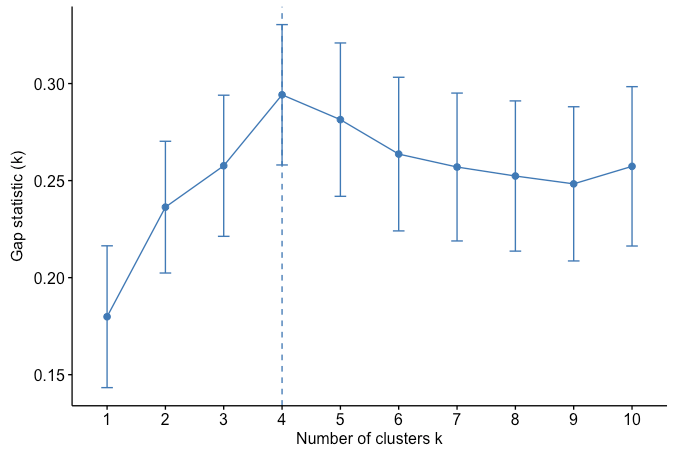
\includegraphics[scale=0.32]{pedro/gapGraph}
		\caption{Ejemplo del método de la brecha \cite{gapGraph}.}
	\end{figure}
\end{frame}

\begin{frame}{Conclusiones}
\begin{itemize}
\item Busca relaciones entre objetos.\break
\item Depende del conjunto de datos, variables seleccionadas, medida de proximidad y método de agrupamiento.\break
\item Métodos jerárquicos: exploratorios, métodos no jerárquicos: confirmatorios.\break
\item Problema: validación de la solución.\break
\end{itemize}
\end{frame}

%%% Parte Práctica

\section{Caso Práctico: \textit{Clustering} en Python}

\begin{frame}{Flor de Iris}

Estudiaremos el conjunto de datos iris de \textbf{Fisher}.\break

Contiene 50 muestras de cada una de tres especies de flor \textbf{Iris}. Para cada muestra, se recogen las medidas de: largo y ancho del sépalo y y largo y ancho del pétalo, en centímetros.

\begin{figure}[h]
  \centering
  \begin{minipage}[h]{0.28\textwidth}
    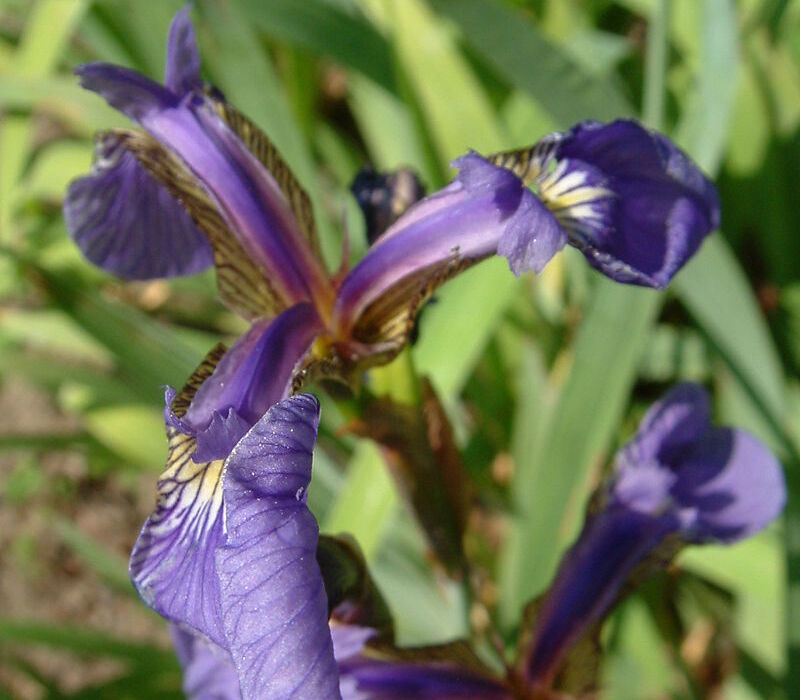
\includegraphics[width=\textwidth]{dani/setosa.jpg}
    \caption{Iris Setosa.}
  \end{minipage}
  \hfill
  \begin{minipage}[h]{0.28\textwidth}
    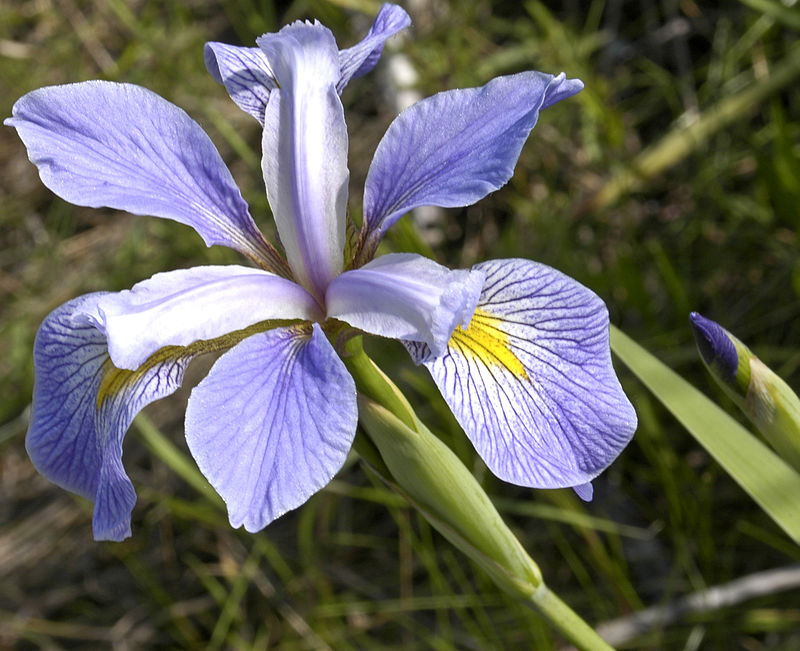
\includegraphics[width=\textwidth]{dani/virginica.jpg}
    \caption{Iris virginica.}
  \end{minipage}
  \hfill
  \begin{minipage}[h]{0.29\textwidth}
    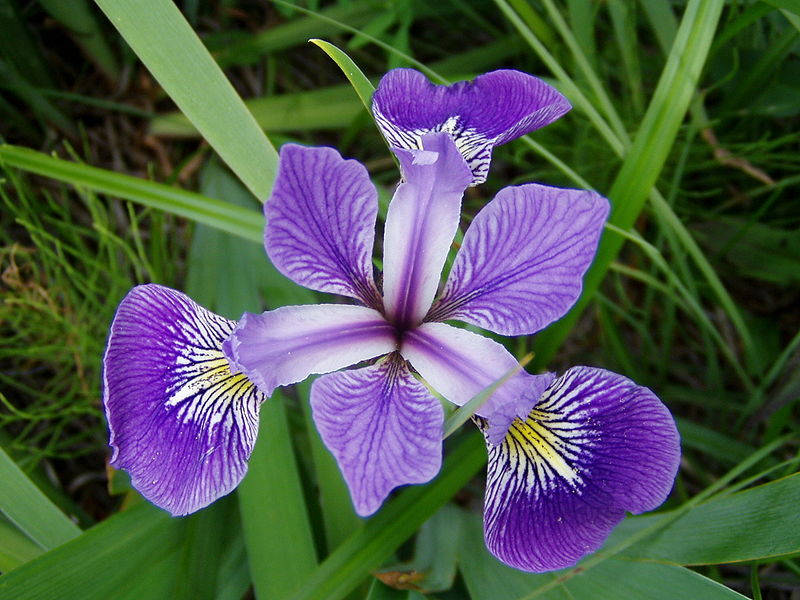
\includegraphics[width=\textwidth]{dani/versicolor.jpg}
    \caption{Iris versicolor.}
  \end{minipage}
\end{figure}
\end{frame}

\begin{frame}{Métricas utilizadas}

Se utilizarán las siguientes métricas para medir la bondad de los algoritmos:\break
\begin{itemize}
\item \textbf{Calinski-Harabaz}: Nos indica si estamos usando un buen número de clústeres para un algoritmo en concreto.\break
\item \textbf{Silhouette}: Cuanto mayor sea su valor, más similar será un objeto respecto a su grupo y más diferente a los de otros clúster. Toma valores entre -1 y +1.
\end{itemize}
\end{frame}

\begin{frame}{Tabla comparativa de los algoritmos}

\begin{table}[H]
\centering
\resizebox{10.5cm}{!} {
\begin{tabular}{lrrrrr}
\toprule
\textbf{Nombre} & \textbf{Nº clústeres} & \textbf{CH} & \textbf{SH} & \textbf{Tiempo ($s$)} & \textbf{Clústeres}                                                                                                          \\ \midrule
K-Means       & 3                    & 359.845074 & 0.504769    & 0.016456      & \begin{tabular}[c]{@{}c@{}}0:    61 (40.67\%)\\
1:    50 (33.33\%) \\2:    39 (26.00\%)\end{tabular}\\ \\
DBSCAN        & 4                   &  94.991819   & 0.306404   &  0.002353      & \begin{tabular}[c]{@{}c@{}}0:    45 (30.00\%)
\\1:    39 (26.00\%)
\\-1:    36 (24.00\%)
\\2:    30 (20.00\%)\end{tabular} \\ \\
AggCluster    & 3                    & 349.254185 & 0.504800    & 0.019058      & \begin{tabular}[c]{@{}c@{}}0:    67 (44.67\%)
\\1:    50 (33.33\%)
\\2:    33 (22.00\%)\end{tabular}                       \\ \\
MeanShift     & 3                    & 290.470683  & 0.476961    & 0.289073      & \begin{tabular}[c]{@{}c@{}}0:    81 (54.00\%)
\\1:    50 (33.33\%)
\\2:    19 (12.67\%)\end{tabular}                                             \\ \bottomrule
\end{tabular}
}
\end{table}
\end{frame}

\begin{frame}[fragile]
\frametitle{K-Means}
Para el algoritmo \textbf{K-Means} se ha utilizado el siguiente código en python y se ha obtenido la siguiente agrupación de las muestras:\break
\begin{lstlisting}
KMeans(init='k-means++', n_clusters=3, 
	n_init=5, random_state=12345)

cluster 0: 61 (40.67%)
cluster 1: 50 (33.33%)
cluster 2: 39 (26.00%)
\end{lstlisting}
\end{frame}

\begin{frame}
\begin{figure}[h]
\centering
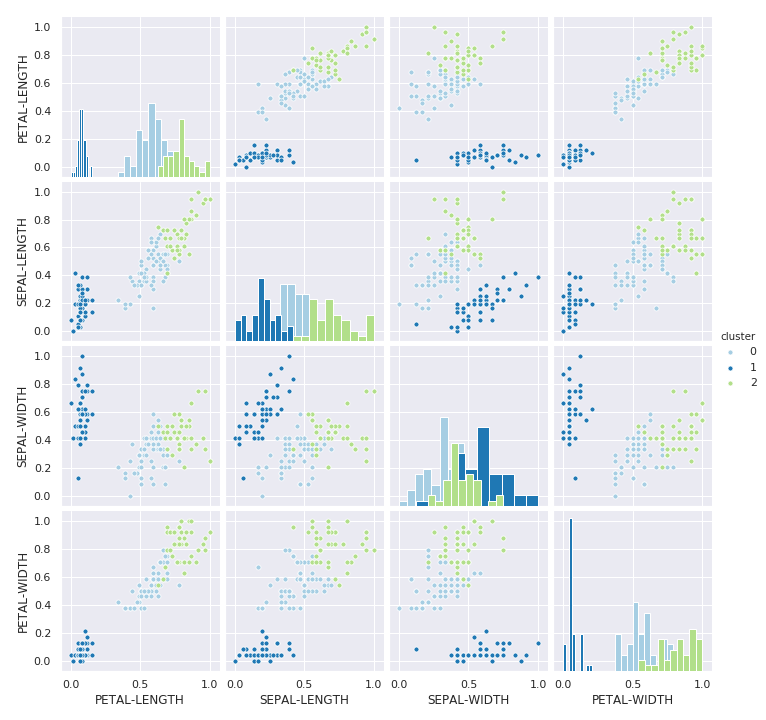
\includegraphics[scale=0.34]{dani/scatmatrixK-MeansIRIS.png}
\end{figure}
\end{frame}

\begin{frame}
\begin{figure}[h]
\centering
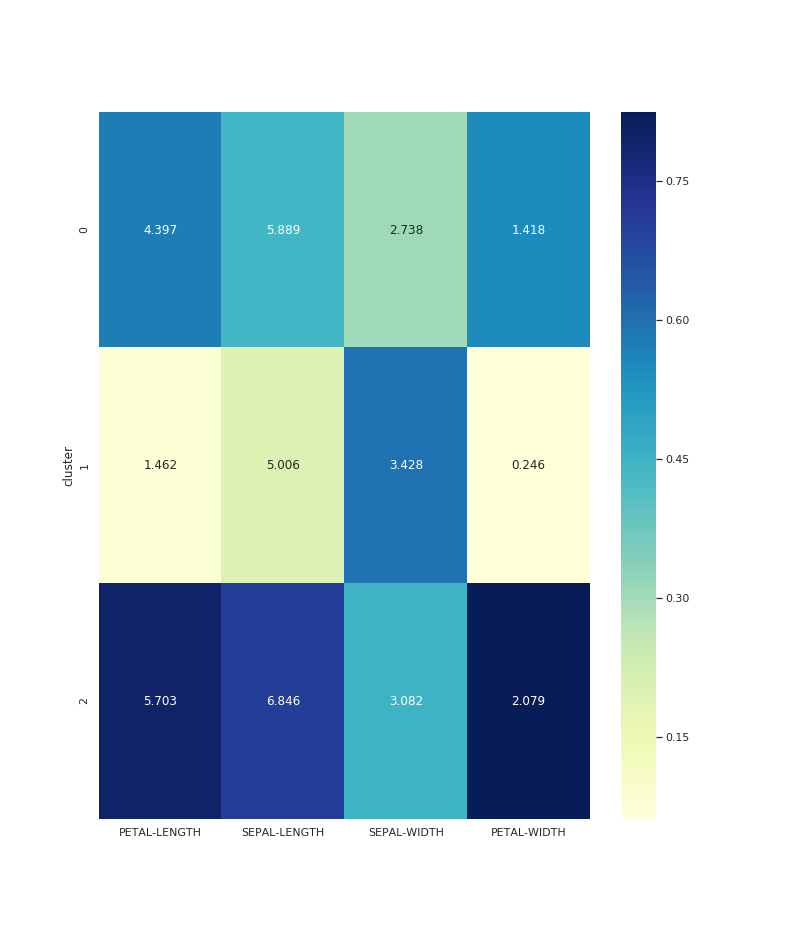
\includegraphics[scale=0.29]{dani/heatmapK-MeansIRIS.png}
\end{figure}
\end{frame}

\begin{frame}[fragile]
\frametitle{Agrupamiento Jerárquico}
Para el algoritmo \textbf{Agglomerative Clustering}, se ha utilizado el siguiente código en python y se ha obtenido la siguiente agrupación de las muestras:\break
\begin{lstlisting}
AgglomerativeClustering(n_clusters=3, 
	linkage="ward", affinity='euclidean')

cluster 0: 67 (44.67%)
cluster 1: 50 (33.33%)
cluster 2: 33 (22.00%)
\end{lstlisting}
\end{frame}

\begin{frame}
\begin{figure}[h]
\centering
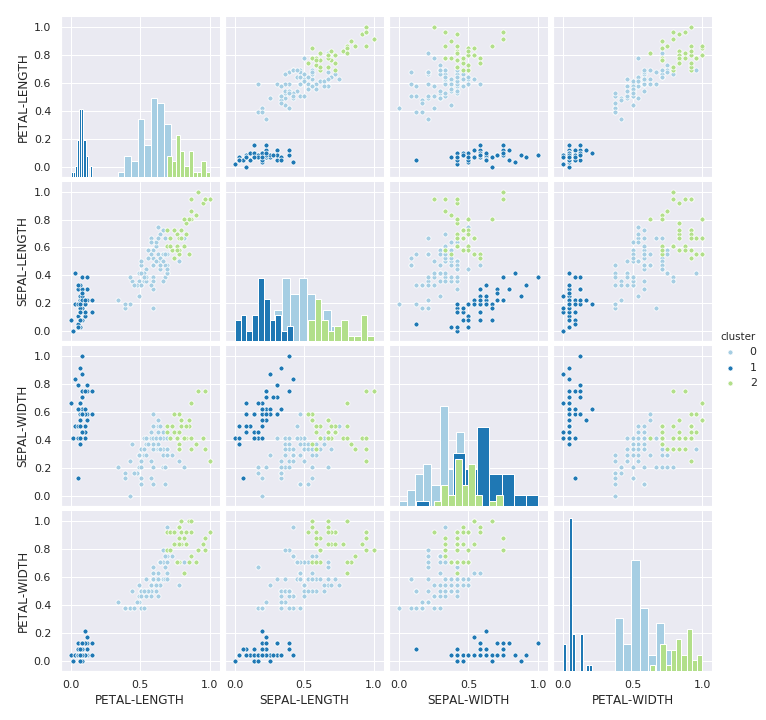
\includegraphics[scale=0.34]{dani/scatmatrixAggClusterIRIS.png}
\end{figure}
\end{frame}

\begin{frame}
\begin{figure}[h]
\centering
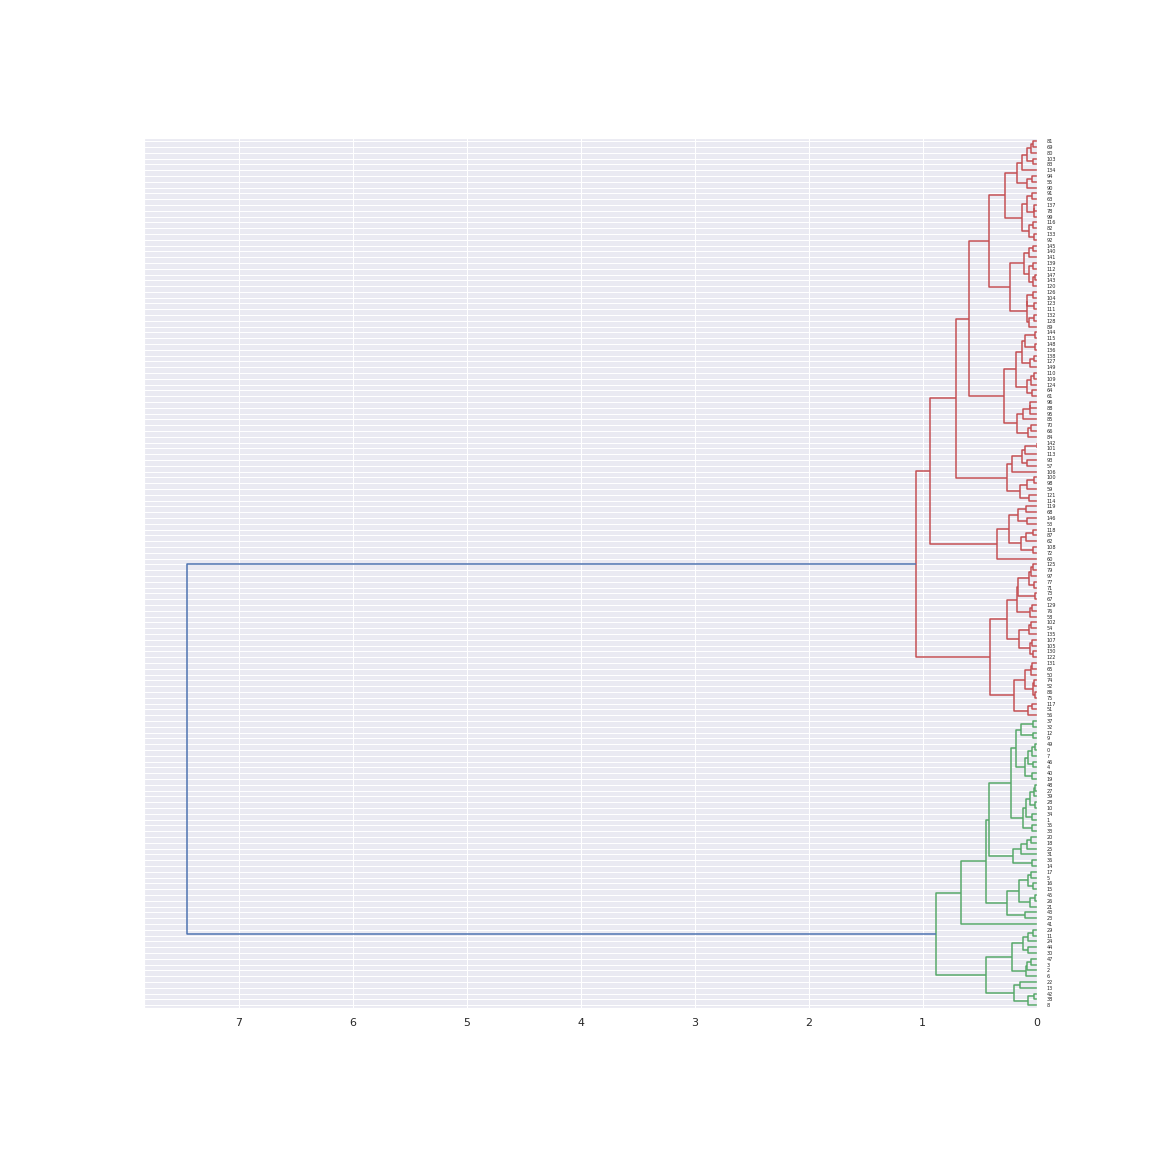
\includegraphics[scale=0.24]{dani/dendrogramAggClusterIRIS.png}
\end{figure}
\end{frame}

\begin{frame}
\begin{figure}[h]
\centering
\textbf{0}: 67 (44.67\%), \textbf{1}: 50 (33.33\%), \textbf{2}: 33 (22.00\%)
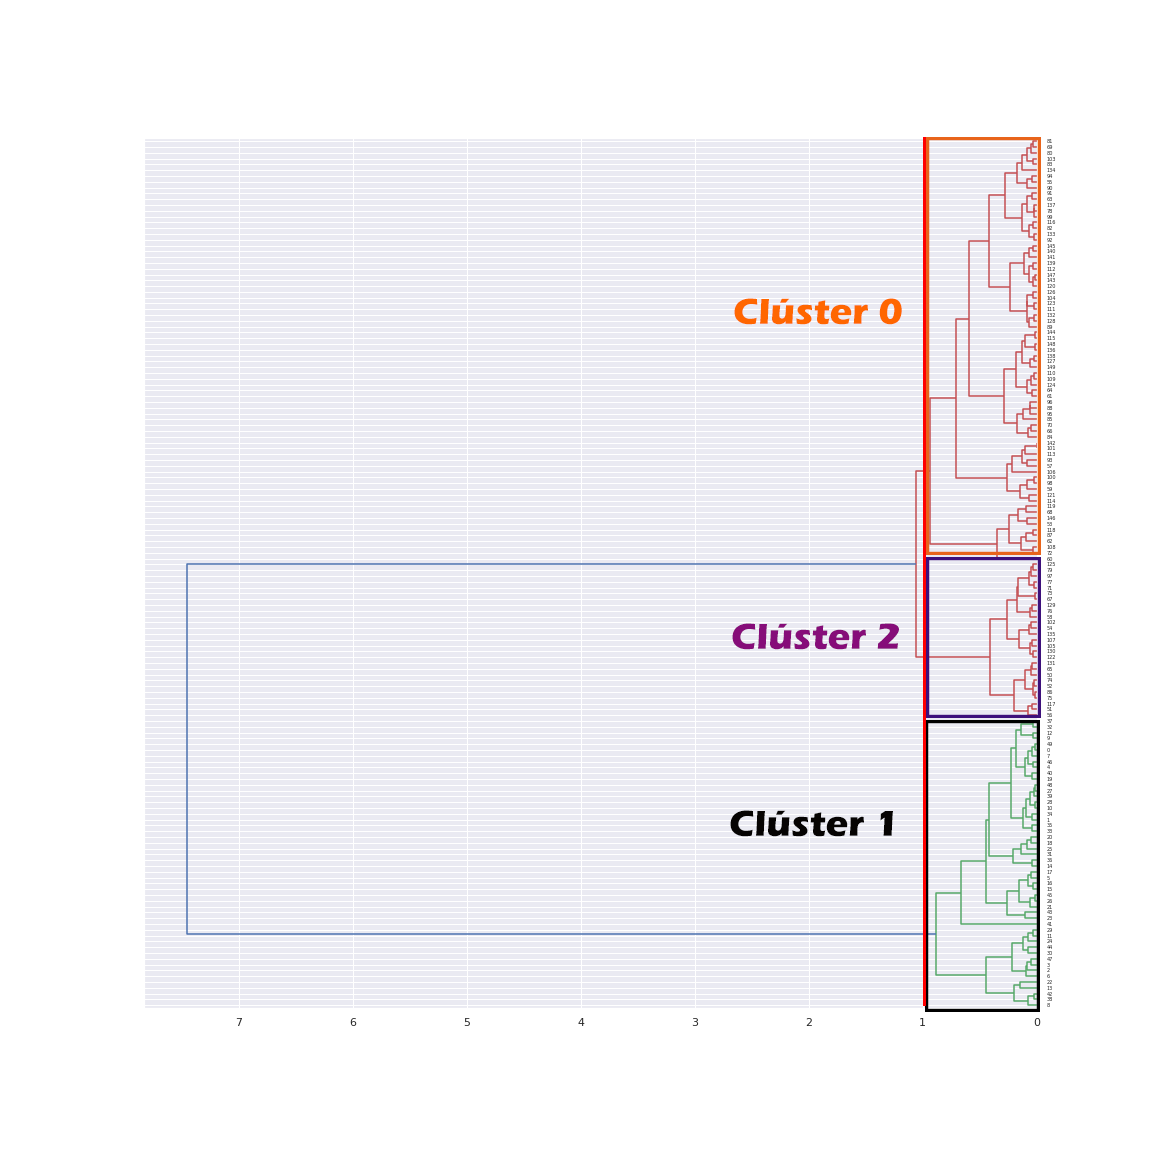
\includegraphics[scale=0.23]{dani/dendrogramcolor.png}
\end{figure}
\end{frame}


\begin{frame}[fragile]
\frametitle{DBSCAN}
Para \textbf{DBSCAN}, se ha utilizado el siguiente código en python y se ha obtenido la siguiente agrupación de las muestras, donde el clúster -1 representa las muestras formadas por ruido:\break
\begin{lstlisting}
DBSCAN(eps=0.12, min_samples=5)

cluster 0:  45 (30.00%)
cluster 1:  39 (26.00%)
ruido  -1:  36 (24.00%)
cluster 2:  30 (20.00%)
\end{lstlisting}
\end{frame}

\begin{frame}
\begin{figure}[h]
\centering
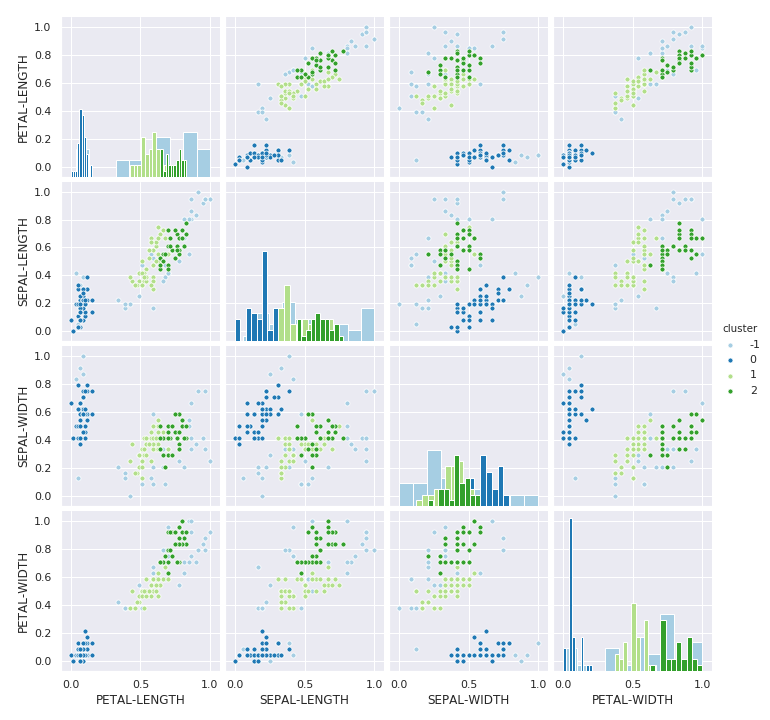
\includegraphics[scale=0.34]{dani/scatmatrixDBSCANIRIS.png}
\end{figure}
\end{frame}

\begin{frame}[fragile]
\frametitle{Mean Shift}
Para \textbf{Mean Shift}, se ha utilizado el siguiente código en python y se ha obtenido la siguiente agrupación de las muestras:\break
\begin{lstlisting}
MeanShift(bandwidth=estimate_bandwidth(X_normal, 
	quantile=0.67, n_samples=400))

cluster 0: 81 (54.00%)
cluster 1: 50 (33.33%)
cluster 2: 19 (12.67%)
\end{lstlisting}
\end{frame}

\begin{frame}
\begin{figure}[h]
\centering
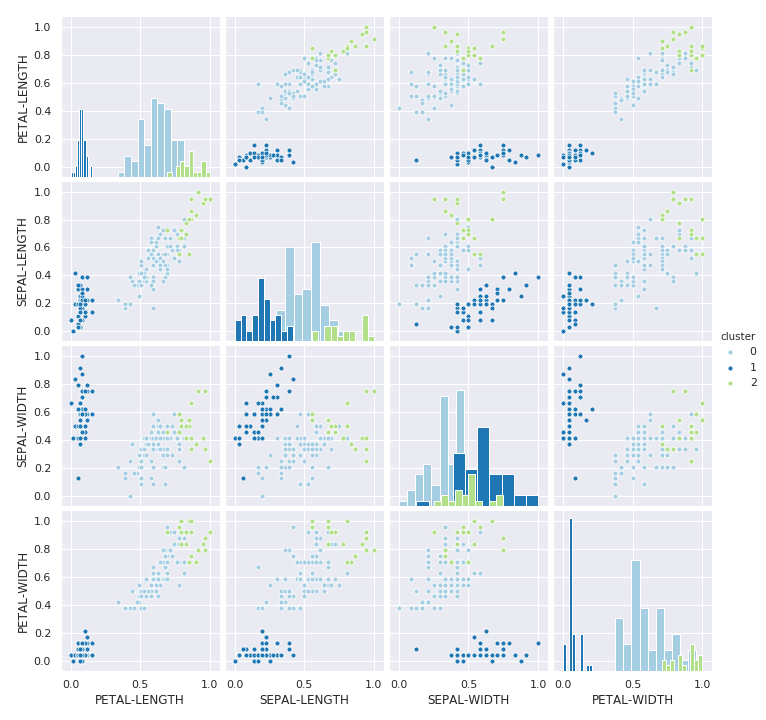
\includegraphics[scale=0.34]{dani/scatmatrixMeanShiftIRIS.png}
\end{figure}
\end{frame}

\begin{frame}[fragile, allowframebreaks]
  \frametitle{Referencias}
%  \nocite{*}
        \bibliographystyle{amsalpha}
        \bibliography{referencias_pres.bib}
\end{frame}
\end{document}

